\cleardoublepage

\section{理论基础 2000字}
我们主要的研究内容是结合图信号处理的理论,设计图卷积神经网络(图2.1)中的图滤波器,
即图卷积层。因此下面部分,我们将简单介绍图卷积神经网络的两种设计方法和他们的相关特点。

\begin{figure}[ht]
    \centering
    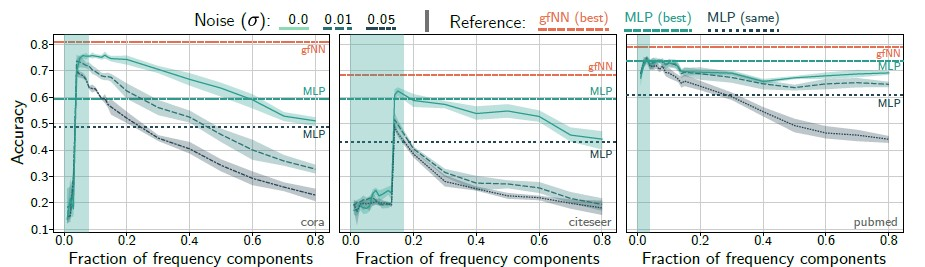
\includegraphics[width=12cm]{theory/1.jpg}
    \caption{\label{2-1}图信号经过图卷积层}
\end{figure}

\subsection{图结构介绍(看字数情况)}

\subsection{基于频谱理论的图卷积神经网络}

\subsubsection{基本理论}
基于频谱的方法在图信号处理中具有坚实的数学基础。用频谱理论来设计图卷积神经网络,默认图是无向的。
由已知的邻接矩阵,我们可以得到归一化的图拉普拉斯矩阵,$ L=I_N-D^{-1/2}AD^{-1/2} $,其中A是邻接
矩阵,D是节点度的对角矩阵 $ D_{ii}={\sum_{j}} A_{ij} $。因为归一化图拉普拉斯矩阵具有
实对称正半定的性质,所以可以将它分解为$ L=U\Lambda U^T $,其中$ U=[u_0,\ldots,u_{n-1}]∈R^{n×n} $
是特征向量的矩阵,$ \Lambda $是特征值的对角矩阵,$\Lambda_{ii}=\lambda_{i} $。归一化拉普拉斯矩阵的
特征向量构成一个标准正交空间,可用$ UU^{T}=I $表示。

在图信号处理中,图信号$ x\in R^n $ 是代表图上所有节点的信号, $ x_i $代表第$ i $个节点
上的信号值。对于信号$ x $,我们可以将它的图傅里叶变换可以表示为,$ F(x)=U^{T}x $,逆变换可以表示为,
$ F^{-1} \widehat{x} = U\widehat{x} $。图傅里叶变换将输入的图信号投影到标准正交空间,在标准正交空间中,
正交基由归一化图的拉普拉斯特征向量构成。变换后的信号$ \widehat{x} $的元素是图信号在新空间中的坐标,
所以输入信号其实就是图傅里叶变换的逆变换,可以表示为$ x = {\sum_{i}}\widehat{x}_{i}u_{i} $。我们可以
将输入信号$ x $与滤波器$ g \in R^{n} $的图卷积被定义为:
$$ x\ast_{G}g = F^{-1}(F(x) \odot F(g)) = U((U^{T}x) \odot (U^{T}g)) $$
其中$ \odot $为元素的阿达玛乘积。所有基于频谱理论的图卷积神经网络都基于上述的定义。如果我们将图滤波器认为
是$ g_{\theta}=diag(U^{T}g) $,那么谱图滤波器可以简化为:
$$ x\ast_{G}g = U g_{\theta} U^{T} x $$
所以基于频谱理论的图卷积网络设计,重点就是如何设计图滤波器$ g_{\theta} $。

\subsubsection{三种主要设计}
初期,在设计图滤波器时,我们直接将图滤波器设计为,$ g_{\theta} = diag(\theta),\theta \in R^n $,则此时的卷积操作
可以表示为,$ y = V g_{\theta} V^{T} x $, 其中$ \theta $为需要学习的参数。这种图滤波器设计方法,缺点是明显的,
当图上节点数量很多(即n的值很大)时,此时将要学习的参数量是很大的,这势必会严重影响图神经网络的效率和表达能力。

后来,为了解决图神经网络的参数过多的问题,又出现了利用特征值矩阵$ \Lambda $的矩阵多项式来设计图滤波器的设计方法。这种方法
将图滤波器表示为,$ g_{\alpha} = {\sum_{i=0}^{K}} \alpha_{i} \Lambda^{i},  \alpha \in R^K $,则此时的卷积操作
可以表示为,$ y = V ({\sum_{i=0}^{K}} \alpha_{i} \Lambda^{i}) V^{T} x $,其中$ \alpha $为需要学习的参数。这种
图滤波器设计方法,明显减少了需学习的参数,但由于计算过程中涉及拉普拉斯矩阵的特征分解,此过程的计算复杂度为$ O(n_{3}) $,
这是非常大的运算开销。

近期,为了提高训练效率,又有人提出了用特征值矩阵$ \Lambda $的Chebyshev多项式来设计图滤波器的方法。这种方法将图滤波器表示
为,$ g_{\beta} = {\sum_{i=0}^{K}} \beta_{i} T_{i}(\Lambda),  \beta \in R^K $,则此时的卷积操作可以表示为,
$ y = V ({\sum_{i=0}^{K}} \beta_{i} T_{i}(\Lambda)) V^{T} x $,其中$ \beta $为需要学习的参数。这种图滤波器设计方法,
不需要学习过多的参数,还避免了拉普拉斯矩阵的特征分解,将计算复杂度降到了$ O(n) $。

\subsubsection{特点}
参考上面部分我们所提到的,基于频谱理论的图卷积神经网络的基本理论和设计方法,我们总结了基于频谱理论的图神经网络的主要特点。
\begin{itemize}
    \item \textbf{无向图} \quad
    因为涉及拉普拉斯矩阵的特征分解,所以频谱理论中适用的图结构必须是无向图。但实际中,还有
    很多有向图的情况,比如交通网络图中,有一些路线可能是只能够单行的。因此,只能处理无向图
    这一特点,很大程度限制了频谱理论在图神经网络的中应用。
    
    \item \textbf{边权重} \quad
    对于频谱理论的设计方法,我们无法学习每条边的权重,邻接矩阵$A$中每条边的权重必须事先确定。
    但是实际中,很多图结构并不是每条连边的权重都是相同的,比如在社交网络中,用户之间的不同关系,
    将直接体现在边权重的不同上。因此,每条边的权重必须事先确定这一特点,限制了基于频谱理论的图神
    经网络的表达能力。

    \item \textbf{泛化能力} \quad
    在基于频谱理论的设计方法中,本质上是用矩阵多项式来拟合图滤波器,那么图结构对拟合的多项式参数
    必然有很直接的影响。然而在现实中,很多图结构并不是固定不变的,比如节点数量的增减和边的连通与否,
    都可能随着时间变化。因此,基于频谱理论的图神经网络并没有很强的泛化能力,这使其不能应用于复杂
    的场景。

    \item \textbf{运算速度} \quad
    基于频谱理论的图神经网络在训练和测试的过程中,主要的运算开销是高阶多项式矩阵需要进行矩阵之间的
    乘法。而在运算过程中,相乘的矩阵大多是稀疏的,并且Chebyshev多项式用矩阵的加减代替了矩阵的乘法。
    因此基于频谱理论的图神经网络的训练速度是较快的。
\end{itemize}

\subsection{基于空间理论的图卷积神经网络}
\subsubsection{基本理论}
与传统CNN在图像上的卷积运算类似,基于空间的方法根据节点的空间关系定义图的卷积。图像可以看作是一种
特殊的图形形式,每个像素代表一个节点。如图2.2a所示,每个像素直接与其附近的像素相连。类似地,基于空
间的图卷积将中心节点的表示与它的邻居的表示进行卷积,以得到中心节点的更新表示,如图2.2b所示。从另一
个角度来看,基于空间的图卷积神经网络与递归图神经网络具有相同的信息传递思想。空间图卷积运算本质上是
沿着边传播节点信息。

\begin{figure}[ht]
    \centering
    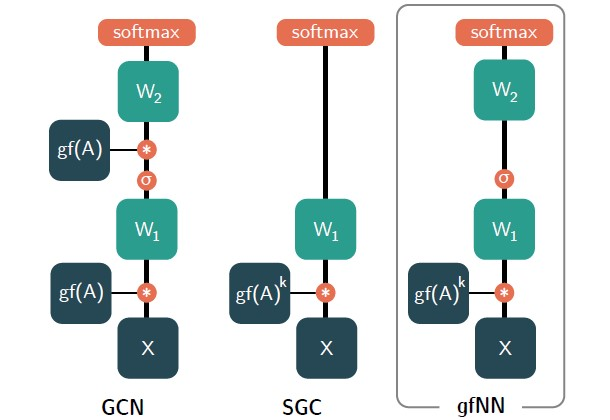
\includegraphics[width=12cm]{theory/2.jpg}
    \caption{\label{2-1}图像上的卷积 vs 图上的卷积}
\end{figure}

注意力机制图神经网络(GAT)是一种最常见的基于空间理论的方法,它假设相邻节点对中心节点的贡献既不完全相同
,也不预先确定,这点与频谱理论非常不同(见图2.3)。GAT采用注意机制来学习两个连接节点之间的相对权重。
根据GAT的图卷积运算定义为:
$$  y = A W x $$
其中,图信号$ x\in R^{F*n} $代表图上所有节点的信号,$ W \in R^{F'*F} $是权重矩阵,$A \in R^{n*n}$是注意力
矩阵,注意力权重衡量节点$i$和它相邻节点$j$的连接权重:
$$
    A_{ij} = \frac{exp(LeakyReLU(\vec{a}^{T}[W\vec{x_{i}}||W\vec{x_{j}}]))}
    { {\textstyle \sum_{k\in N_{i} }^{}} exp(LeakyReLU(\vec{a}^{T}[W\vec{x_{i}}||W\vec{x_{k}}]))}  
$$
其中,$\vec{a} \in R^{2F'}$是一个需要学习的矢量参数,$ || $是一个将两个向量拼接的运算,$ N_{i} $表示节点$i$的
相邻的节点,softmax函数保证了节点$i$所有邻居的注意权值总和为$1$。此外,GAT实现了多部分注意机制,进一步提高了模
型的表达能力。

\begin{itemize}
    \item \textbf{有向图} \quad

    
    \item \textbf{边权重} \quad


    \item \textbf{图结构的hop} \quad


    \item \textbf{运算速度} \quad

\end{itemize}

\subsubsection{特点}